\documentclass[11pt,letterpaper]{article}
\usepackage{graphicx}
\usepackage{geometry}
\usepackage{amsmath}
\usepackage{amssymb}
\usepackage{hyperref}
\usepackage{url}
\usepackage{xurl}
\usepackage{natbib}
\usepackage{booktabs}
\usepackage{xcolor}
\usepackage{listings}
\usepackage{array}
\geometry{margin=1in}
\hypersetup{colorlinks=true, linkcolor=black, citecolor=black, urlcolor=black}

\newtheorem{proposition}{Proposition}

\title{Catching Edited Safety Models by Reading Weights in Sliding Windows}
\author{}
\date{}

\begin{document}
\maketitle

\begin{abstract}
Deciding whether an open-weight checkpoint still has its safety training intact normally costs a benchmark run: hundreds of harmful prompts, a judge model, and a repeat per attack template. A parent-free weight statistic can replace that at zero prompts and zero forward passes --- it reads the smallest eigendirection of the pooled residual-write Gram matrix and asks whether some layer is annihilated along it --- but pooled over the whole stack it reaches only 0.159 sensitivity on 44 real edited Hub checkpoints from 27 uploaders, because a depth-localised edit is diluted by untouched layers until the removed direction never becomes the Gram's minimal direction, at which point the statistic returns its parent's value however completely the edited layers were annihilated. We show that the failure is a pooling artefact and remove it. Computing the statistic on sliding windows of $k$ consecutive layers and scoring the checkpoint by the extremum over windows --- a construction containing the pooled statistic exactly as its $k=L$ special case --- raises sensitivity on 50 real edited checkpoints from 0.300 [0.191, 0.438] to 0.700 [0.562, 0.809] at specificity 1.000 on 57 eligible undeclared negatives, recovering the partial-layer (0.80 vs 0.00), multi-direction (0.80 vs 0.00), merge (0.75 vs 0.00) and per-component (0.62 vs 0.12) recipes that dominate the Hub, and tying an 11-term repository-name regex while reading no name. Two boundaries are analytic rather than empirical: a sub-unit uniform kernel fails completion at every window size, and an isometric Householder edit leaves the Gram spectrum exactly invariant and is provably invisible to every statistic in this family. We also show, by building the checkpoints rather than by correlation, that the weight verdict and safety behaviour dissociate in both directions --- an edit that un-censors from 0.950 to 0.270 reads its parent's value to four decimals, and an edit reading $-4.587$ refuses at its parent's rate --- so no such certificate may be read as a safety score.
\end{abstract}

\section{Introduction}

An open-weight checkpoint arrives with no provenance. Deciding whether its safety training is intact currently costs a benchmark run: hundreds of harmful prompts from AdvBench \citep{Zou2023}, JailbreakBench \citep{Chao2024} or HarmBench \citep{Mazeika2024}, a judge model to score the generations \citep{Zheng2023}, and a repeat for every attack template of interest. At the scale of a model hub that unit of cost is wrong. A harvest of 61 Hub sweeps over 20,313 enumerated repositories finds 513 self-declared edited checkpoints from 189 distinct uploaders below 4.2B parameters alone, and a follow-up census returns 1,068 hits of which 116 are sub-4.2B\footnote{Code: \url{https://github.com/AMGrobelnik/ai-invention-c9546e-rating-model-safety-in-eighty-forward-pa/tree/main/round-4/research-1}}.

The published cheap alternatives each retain a dependency the situation does not grant. Activation-geometry scanners need harmful prompts \citep{Messenger2026}; refusal-alignment scores need unsafe prompts, jailbreak prompts \emph{and} a safety-aligned reference model \citep{Huang2026}; weight-space safety-basin volume needs a harmful benchmark evaluated at every perturbation \citep{Peng2024}. The two closest weight-space results both require the parent: the abliteration audit of \citet{Hurtado2026}, whose statistic is the rank-one energy fraction $E_1 = \mathrm{mean}_m\,\sigma_1^2(\Delta W_m)/\sum_i \sigma_i^2(\Delta W_m)$ with $\Delta W = W_{\text{base}} - W_{\text{cand}}$, band-averaged over a fixed mid-stack band and credited to the WeightWatch primitive \citep{Zhong2025}; and the spectral-geometry study of LoRA adapters \citep{Paul2026}. A random repository does not come with an attested parent.

The parent-free substitute is straightforward to state. If abliteration \citep{Arditi2024, Labonne2024} projects one direction out of every residual-write matrix, that direction becomes a shared approximate null direction of the write ensemble and should be recoverable from the ensemble alone. Let $\mathcal{W}$ be the residual-write matrices (attention output projections and MLP down-projections) over all $L$ layers, $A = \sum_{W} WW^\top/\lVert W\rVert_F^2$ the shared Gram matrix, $v_1$ its minimum eigenvector, and $e_W(u) = \lVert u^\top W\rVert^2/(\lVert W\rVert_F^2/d)$ the normalised write energy along a unit direction $u$. The pooled statistic is
\[
W05 \;=\; \log_{10}\ \min_{W\in\mathcal{W}}\ e_W(v_1).
\]
It costs zero prompts, zero forward passes and roughly 7--11\,s of CPU linear algebra, and it separated 8 abliterated from 36 non-abliterated archived checkpoints at oriented AUROC 1.000.

\textbf{That statistic does not survive contact with the Hub, and this paper's positive result is the fix.} On 44 real public sub-4.2B edited checkpoints from 27 uploaders across 9 recipe classes, the pooled statistic at its panel-fitted operating point fires on 7 --- sensitivity 0.159 --- while its five archived calibration positives all still fire\footnote{Code: \url{https://github.com/AMGrobelnik/ai-invention-c9546e-rating-model-safety-in-eighty-forward-pa/tree/main/round-4/experiment-1}}. The failure is not noise: \texttt{mlabonne/Qwen3-0.6B-abliterated} reads $-0.9637$ against its own parent's $-0.9641$, a paired shift of $4\times10^{-4}$.

The reason is \emph{pooling}. The Gram matrix sums over the whole stack, so a depth-localised edit is diluted by the untouched layers and the removed direction never becomes the Gram's minimal direction. Whenever that happens the statistic returns the parent's value exactly, and the completion of the edit is irrelevant: over a nine-point Gaussian depth sweep with the host and the removed direction $r$ held fixed, the peak layer is annihilated \emph{completely at every spread} ($\log_{10}\min_W e_W(r) = -4.53$ throughout) while $W05$ sits at the parent's $-1.0098$ for every spread up to 4 and only crosses threshold between spread 8 and 16, exactly where the kernel's \emph{minimum} depth weight rises from 0.0796 to 0.5311 and $|\cos(v_1,r)|$ jumps from 0.126 to 0.9992\footnote{Code: \url{https://github.com/AMGrobelnik/ai-invention-c9546e-rating-model-safety-in-eighty-forward-pa/tree/main/round-5/evaluation-1}}.

\begin{figure}[!htbp]
  \centering
  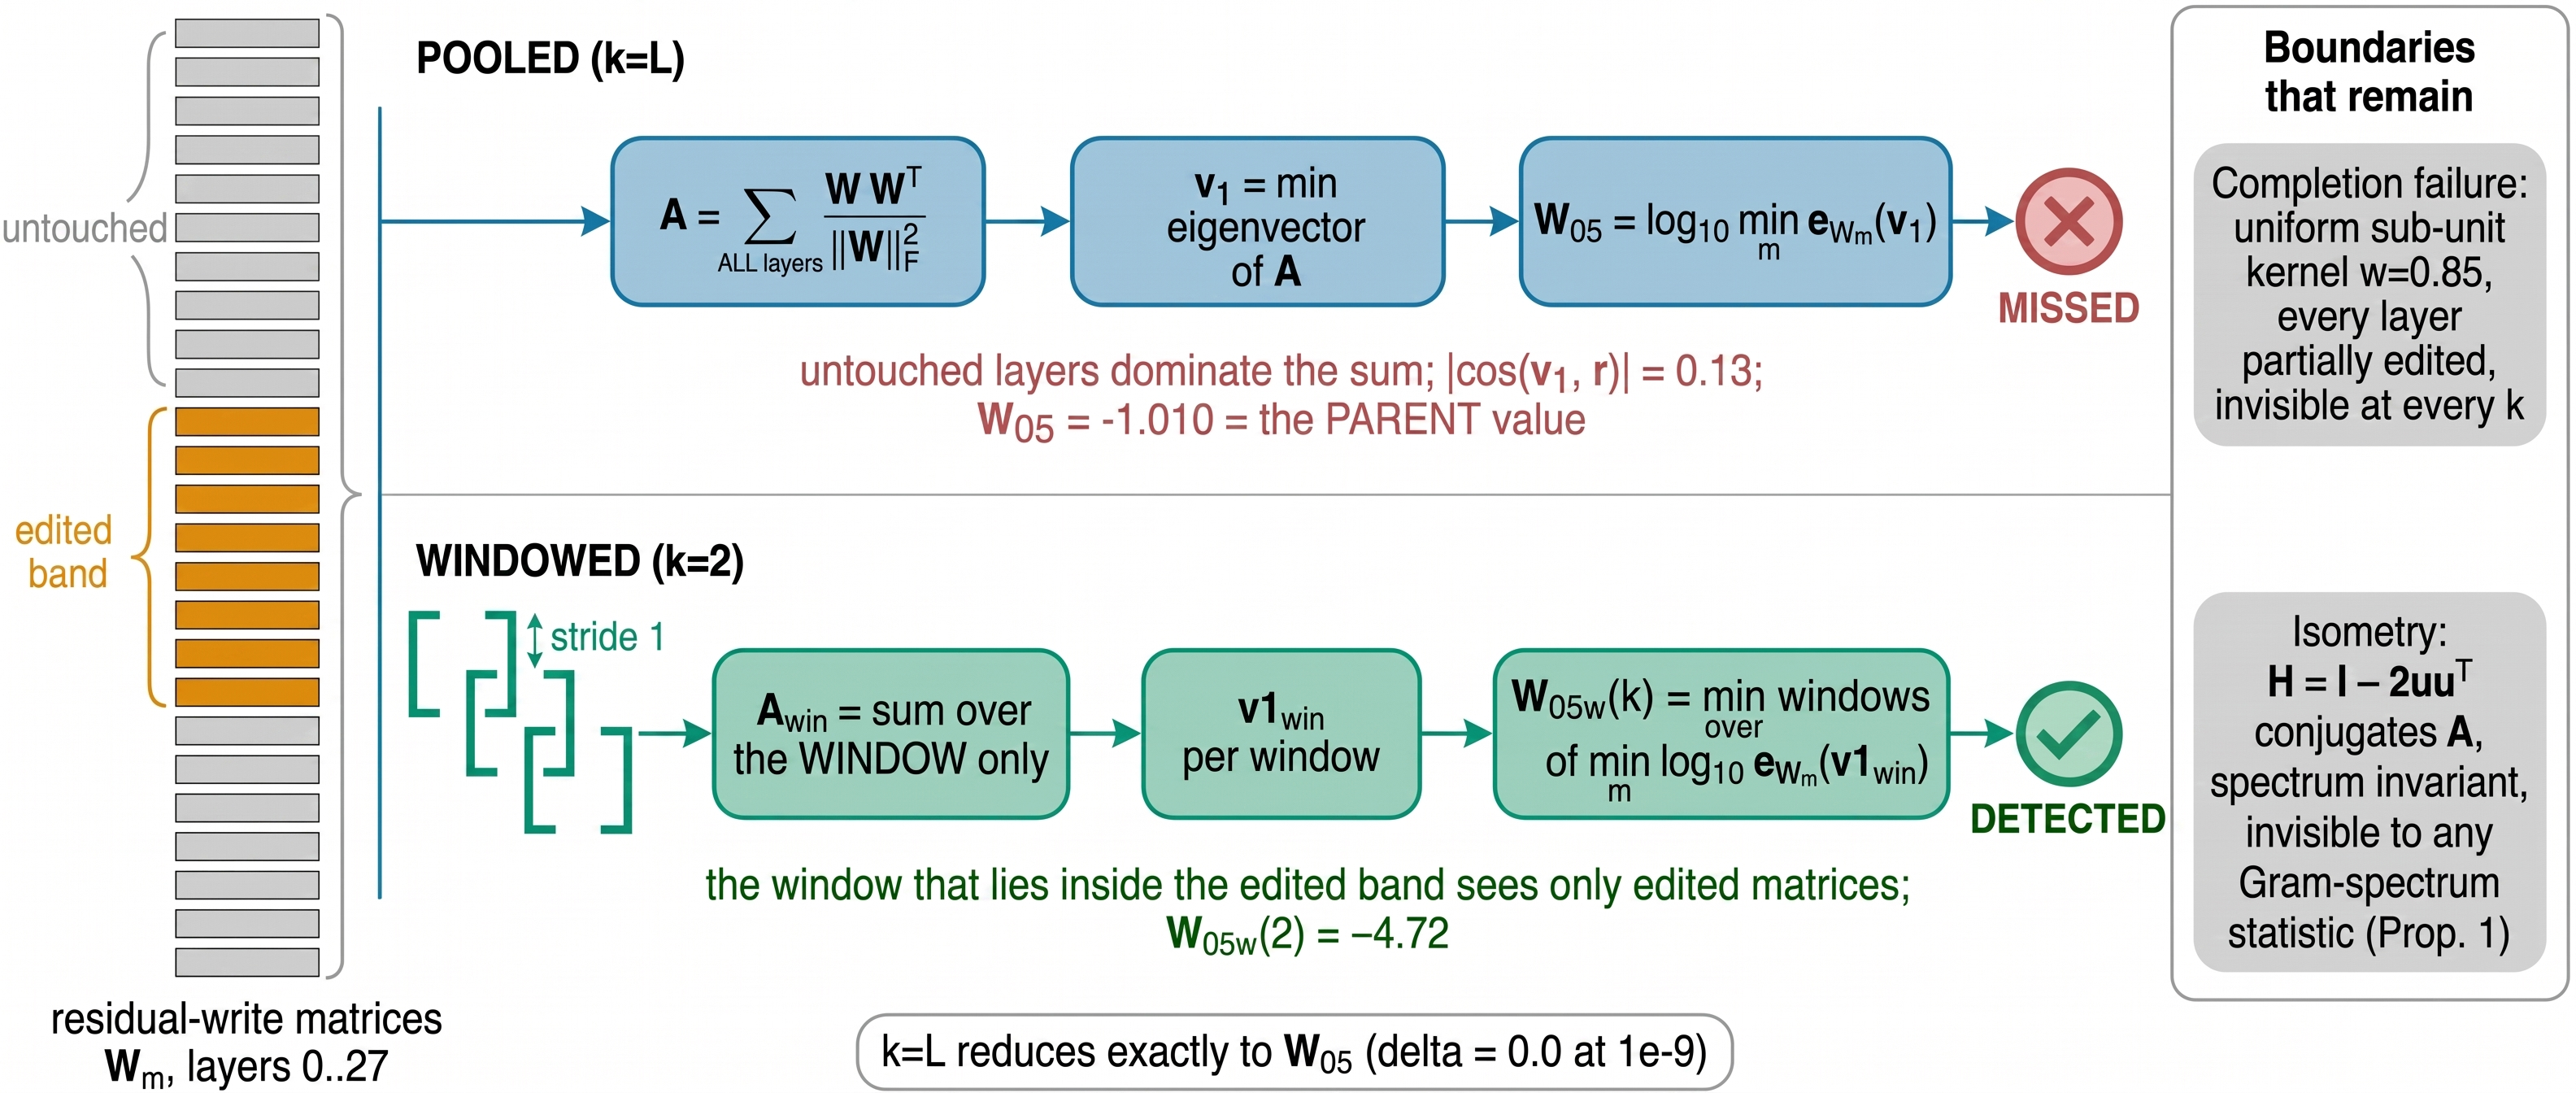
\includegraphics[width=\linewidth,height=0.85\textheight,keepaspectratio]{figures/fig1_v0.jpg}
  \caption{The mechanism and the remedy. Left: a depth-localised abliteration edits a contiguous band of residual-write matrices, but the shared Gram matrix sums over all $L$ layers, so the untouched layers dominate and the removed direction $r$ never becomes the Gram's minimal eigenvector $v_1$; the pooled statistic $W05$ then returns the unedited parent's value. Right: computing a minimum eigenvector inside each sliding window of $k$ consecutive layers and scoring the checkpoint by the extremum over windows surfaces the edit. At $k=L$ a single window covers the stack and the construction reduces exactly to $W05$. Two boundaries remain by construction: a sub-unit uniform kernel fails completion at every $k$, and an isometric (Householder) edit leaves the Gram spectrum invariant and is invisible to every member of the family.}
  \label{fig:fig1}
\end{figure}

Because the blind spot is a pooling artefact, the fix is to stop pooling. We define $W05w(k)$ on sliding windows of $k$ consecutive layers, take the minimum eigenvector \emph{within each window}, and score the checkpoint by the extremum over windows; at $k = L$ a single window covers the stack and $W05w(L) \equiv W05$, so the pooled statistic is a special case rather than a competitor. Scored on 50 real edited Hub checkpoints against 57 eligible undeclared negatives, and with every threshold matched to specificity 1.000 on the negatives, \textbf{$W05w(k{=}2)$ reaches sensitivity 0.700 [0.562, 0.809] where the pooled statistic reaches 0.300 [0.191, 0.438]} --- more than double the recall at zero false positives (Figure~\ref{fig:fig2}). It ties an 11-term regex over the repository identifier (0.700) and beats that regex's frozen 8-term ancestor (0.580) while reading no repository name at all, which matters because a name regex is a \emph{declaration} detector and cannot fire on an undeclared edit by construction. The classes it recovers are the ones that dominate the Hub: partial-layer 0.80 against 0.00, multi-direction SVD 0.80 against 0.00, merge-of-abliterated 0.75 against 0.00, Heretic per-component 0.62 against 0.12, uncensoring SFT 0.62 against 0.00.

The recovery has a boundary and the boundary is analytic, not empirical. Two failure classes are provably out of reach. \emph{Completion failures} --- a uniform sub-unit projection at weight $w \in \{0.5, 0.7, 0.85\}$ that leaves every layer partially edited --- are invisible at every $k$ and every consistency threshold, because windowing changes the \emph{scope} of pooling and never the \emph{completeness} of a removal; at $w = 0.85$ the edit is as behaviourally effective as the full one (harmful refusal 0.225 against 0.200) and still invisible. \emph{Isometric edits} are worse than hard: a Householder reflection $H = I - 2uu^\top$ applied to every write matrix conjugates $A \mapsto HAH^\top$ and leaves its spectrum exactly invariant, so \textbf{no statistic reading that spectrum can see it, windowed or pooled} (Proposition~\ref{prop:iso}). Measured, ORBA's Householder recipe moves $W05$ by $4.1\times10^{-5}$ --- \emph{less} than a Householder about an unrelated random direction moves it ($7.3\times10^{-5}$) --- while dropping harmful refusal to 0.100.

Two further results are decisive for anyone who would deploy such a certificate. First, the weight verdict and the safety behaviour are dissociable \textbf{in both directions, by construction rather than by correlation}\footnote{Code: \url{https://github.com/AMGrobelnik/ai-invention-c9546e-rating-model-safety-in-eighty-forward-pa/tree/main/round-4/experiment-3}}: a depth-weighted Gaussian abliteration of Qwen3-1.7B built with the refusal direction held fixed un-censors from 0.950 to 0.270 [0.196, 0.360] at $n = 111$ while reading $W05 = -1.0100$, its unedited parent's value to four decimals; and a uniform abliteration of Llama-3.2-1B-Instruct along the AUROC-argmax direction fires the full signature at $W05 = -4.587$ while refusing at its parent's 0.950. Second, the operating point is arbitrary: holding out one recipe class refits the threshold from $-2.7415$ to $-1.7156$, a shift of 1.026 log-units and 8.04 times the 0.128-log-unit shift that already produces a first false positive; and while the panel threshold gives 0 false positives on 251 eligible undeclared checkpoints (159 of them chat-templated), the refit threshold gives 20\footnote{Code: \url{https://github.com/AMGrobelnik/ai-invention-c9546e-rating-model-safety-in-eighty-forward-pa/tree/main/round-5/experiment-2}}.

\subsection{Summary of Contributions}

\begin{itemize}
  \item \textbf{A windowed parent-free edit detector that more than doubles real-checkpoint recall} (\S\ref{sec:windowed}): $W05w(k{=}2)$ 0.700 [0.562, 0.809] against pooled 0.300 [0.191, 0.438] on 50 real edited Hub checkpoints at specificity 1.000, recovering partial-layer, multi-direction, merge and Heretic classes the pooled statistic never touches, at zero prompts and zero forward passes.
  \item \textbf{An analytic characterisation of what parent-free spectral detection can and cannot reach} (\S\ref{sec:theory}): discovery and completion are the same quantity to within a Cauchy--Schwarz bound whenever discovery holds, so the operative content is \emph{which} kernels achieve discovery; windowing repairs discovery failures whose edited band is at least $k$ layers wide, and Proposition~\ref{prop:iso} proves isometric edits permanently invisible to any Gram-spectrum statistic, windowed forms included.
  \item \textbf{A both-directions dissociation between the weight signature and safety behaviour, built as checkpoints} (\S\ref{sec:operating}): un-censored at the parent's $W05$, and signature-positive at the parent's refusal rate --- each with intervals, and each surviving re-scoring by an independent judge from a different model family.
  \item \textbf{A de-biased measurement of the baseline the field would actually use} (\S\ref{sec:name}): the repository-name regex scores 0.953 [0.925, 0.970] on checkpoints discovered by name search and 0.642 [0.507, 0.757] on checkpoints discovered name-free, so the widely quoted number is an upper bound; and on the 34 edited checkpoints the regex cannot see, the pooled statistic fires 0 times.
\end{itemize}

\section{Related Work and Positioning}

\paragraph{Parent-requiring weight audits.} WeightWatch \citep{Zhong2025} shows that top singular vectors of a fine-tuned-minus-base difference correspond to newly acquired behaviours, and is the primitive on which the abliteration audit of \citet{Hurtado2026} builds its $E_1$. Primary-source reading establishes that $E_1$ is \emph{already} band-averaged over ``each layer in the mid-stack band $B$'', so per-band scoring of a weight statistic is published prior art and we concede it. The spectral-geometry study of LoRA adapters \citep{Paul2026} reaches binary drift AUC 1.00 on 38 manufactured adapters; two of its five features are formula-identical to auxiliary statistics we do not rely on, and its single most informative feature is a cosine to a \emph{healthy-adapter centroid}, requiring both a parent and a reference population. Its cross-method AUC 0.00 result ($n_{\text{bootstrap}} = 972$) is the strongest published precedent for a recipe boundary, and must be carried with the confound the paper declares itself: its steering arm produced incoherent text at every intensity, GPT-4o scoring 0 of 300 responses harmful. Backdoored-LoRA detection from weights alone \citep{BackdooredLoRA2026} operates at our size class, but on an adapter already separated from a frozen base, with supervised calibration on labelled adapters.

\paragraph{Community weight forensics is further along than an academic reading suggests, and it supports our mechanism.} Abliterlitics \citep{Sapwell2026} is an open-source abliteration-forensics toolkit (AGPL-3.0, first public 2026-04-24) with published reports on ten base models from ${\sim}$2B to 59B. Every one of its weight metrics is computed on the \emph{delta}: its methodology is literally \texttt{diff = (variant - base).abs().mean()} and \texttt{svd(delta\_matrix)}, its documented usage requires ``a directory with your base model and variants, plus a \texttt{comparison.json}'' with \texttt{base} a mandatory key, and it has no single-checkpoint mode\footnote{Code: \url{https://github.com/AMGrobelnik/ai-invention-c9546e-rating-model-safety-in-eighty-forward-pa/tree/main/round-5/research-1}}. It is therefore parent-requiring, which sharpens rather than blunts our claim --- and its measurements are the strongest \emph{external} evidence for the depth-versus-completeness decomposition this paper recovers without a parent. Four of its reports sit at or below ${\sim}$4.5B, including a full weight report on the Qwen3-4B family we study. On a shared Qwen3.5-9B base, Heretic modifies 23 of 32 layers with layers 0--8 untouched, HauhauCS 29 and Huihui 31, while Heretic and Huihui agree almost perfectly in \emph{direction} (median cosine 1.0, global mean 0.997). The recipes differ in depth and completeness, not in direction. We present our mechanism as an independent, parent-free confirmation of what delta-based forensics measures, not as a discovery. The one caveat we must carry with the cosine agreement is that the same Heretic--Huihui pair is essentially orthogonal (median cosine 0.00017) on Qwen3.5-4B, so 0.997 is a property of one base and not of the pair.

\paragraph{Parent-free spectral statistics that are not edit detectors.} The nearest work carries three of our four qualifiers and must be ruled out on the record. A random-matrix analysis of transformer spectra \citep{Staats2024} is parent-free, calibration-free and reads the \emph{bottom} of the spectrum, establishing that departures from the Marchenko--Pastur null appear among the smallest singular values and that removing them costs more perplexity than removing bulk values --- but it asks where information is stored, not whether a checkpoint has been edited, and it is not windowed. EigenTrack \citep{Ettori2025} is a sliding spectral detector, but it slides over \emph{time} across activations rather than over \emph{depth} across weights. Spectral Signatures \citep{Zhang2026} is parent-free but designed so that ``the impact of post-training on the weight ESD is minimal'', which is exactly the wrong property for an edit detector, and its estimator reads the top $n/2$ eigenvalues. The Intruder Threshold \citep{Xie2026} derives a critical LoRA update strength from the pretrained spectrum alone but compares it against $\sigma_1(BA)$, so it needs the update matrix and reads the top of the spectrum; it is a law about when training creates intruder dimensions, not a detector of a completed edit. Weight-homology identification and output-geometry fingerprinting answer lineage, not edit detection. The only \emph{shipped} parent-free abliteration detector we could find, \texttt{reverse-abliterate} \citep{ReverseAbliterate}, reads filenames and metadata and no tensor values; it is the software instantiation of the repository-name baseline \S\ref{sec:name} measures. Our novelty claim is therefore narrow and explicit: the conjunction of parent-free, calibration-free, bottom-of-spectrum and sliding-window-with-extremum scoring, of which the fourth qualifier is earned in \S\ref{sec:windowed} by measurement rather than asserted by construction.

\paragraph{The recipe family, read from source.} Abliteration is not one operation. Heretic's kernel is a \textbf{triangular tent with a hard cutoff}, not the Gaussian that its own downstream documentation asserts: \texttt{if distance > min\_weight\_distance: continue}, followed by linear interpolation, with \texttt{max\_weight\_position} sampled in $[0.6L, 1.0L]$ and \texttt{direction\_index} in $[0.4L, 0.9L]$, so the peak is \emph{code-level forbidden} from the early stack \citep{Weidmann2026} --- a prediction that matches Abliterlitics' independent measurement that layers 0--8 carry no real edits. Heretic's shipped default is already norm-preserving. OBLITERATUS \citep{Obliteratus2026} ships a \emph{spectral certification} step, but its source settles that it consumes \textbf{activations}: \texttt{certify(harmful\_activations, harmless\_activations, layer\_idx)} thresholds eigenvalues of a between-class rank-one outer product against a Baik--Ben Arous--P\'ech\'e bound. It is parent-free but not prompt-free, and it audits an edit the operator just performed; being layer-selective via COSMIC \citep{Siu2025}, its rank-$k$ presets are \emph{degraded}, not detected. ORBA \citep{Lai2026} is two distinct recipes: at $\lambda = 1$ the operation is annihilation \emph{without} reflection, while only the v3 Householder is a true isometry --- conflating them makes the falsification in \S\ref{sec:boundaries} vacuous, which is why we implement and report both. The remaining members are the depth-weighted Gaussian kernel \citep{Labonne2024}, MPOA's exact four-step row-norm-preserving update \citep{Lai2025}, Gabliteration's ridge-regularised rank-$k$ update \citep{Guelmez2026}, concept-registry ridge residualisation \citep{Cristofano2026}, and behavioural SFT, which has no closed form. A cross-architecture comparison exists \citep{Young2025} but evaluates at 7B--14B.

\paragraph{Why a scar is expected, and why detection is not control.} Safety fine-tuning minimally transforms MLP weights so as to align unsafe inputs into a null space \citep{Jain2024}, safety behaviour localises to a small set of neurons and ranks \citep{Wei2024}, and abliteration's off-target effects are documented \citep{Agnihotri2025, Fafula2026}; extended-refusal training defends against abliteration while leaving weights superficially normal \citep{Shairah2025}. The general dissociation between detecting a behaviour and controlling it is published \citep{Galeone2026} --- a linear detector at AUC 1.000 sitting at $\cos = 0.12$ from the direction that produces the behaviour --- and its Section 8 makes cosine-as-safety-score a published negative. \S\ref{sec:dissoc} reports the same dissociation where the ``detector'' is a weight statistic, in both directions and by construction. Finally, safety alignment is concentrated in the first few generated tokens \citep{Qi2024}, and interpretability results report near-perfect internal decodability alongside far weaker output sensitivity \citep{Basu2026}: a read-side metric can be confidently wrong about behaviour.

\section{Panel, Statistic and the Analysis Contract}

\subsection{The statistic and its windowed generalisation}

With $A$, $v_1$, $e_W(\cdot)$ and $W05$ as defined in \S1, the windowed statistic takes windows of $k$ consecutive layers with stride $\max(1, \lfloor k/2\rfloor)$, drops the ragged tail, computes a per-window minimum eigenvector $v_1^{\text{win}}$ of the Gram accumulated over that window's matrices only, and scores
\[
W05w(k) \;=\; \min_{\text{win}}\ \min_{m\in\text{win}}\ \log_{10} e_{W_m}\!\left(v_1^{\text{win}}\right), \qquad c(k)=\min_{\text{adj}}\left|\cos\!\left(v_1^{\text{win}_i}, v_1^{\text{win}_{i+1}}\right)\right|,
\]
with $c(k)$ available as a consistency gate swept over a threshold. At $k = L$ one window covers the stack, so $W05w(L) \equiv W05$ by construction, and this identity is used as a built-in reproduction gate (\S\ref{sec:contract}). Auxiliary statistics $W01 = \log_{10}(\mathrm{median}(\lambda)/\lambda_1)$ and $W04 = \log_{10}(\lambda_2/\lambda_1)$ appear in earlier work on this statistic family and are \textbf{retired from any load-bearing role here}: both are log ratios against $\lambda_1$, which on an abliterated checkpoint sits at the float32 Gram-accumulation floor, and on bit-identical weights they are irreproducible below ${\sim}0.05$ while $W05$ reproduces to $1.3\times10^{-5}$.

\subsection{Panels}

Four panels are used and never mixed. (P1) The \textbf{archived battery panel}: 44 checkpoints at $\leq 4.2$B over 23 weight lineages and 7 architecture families, comprising 16 base, 15 instruct, 8 abliterated, 4 behaviourally-uncensored and one safety-RL checkpoint. (P2) The \textbf{at-scale recipe panel}: 44 real public sub-4.2B edited checkpoints from 27 uploaders across 9 recipe classes, plus 20 freshly measured Hub parents as negatives, extended this iteration to 50 scored edited checkpoints for the windowed arm and to 84 for the baseline arm, plus 47 in-house kernels on a fixed host with a fixed direction. (P3) The \textbf{wild panel}: undeclared Hub checkpoints filtered by a pre-stamped eligibility rule --- 251 eligible rows for the pooled statistic (159 chat-templated, 78 base, 14 unlabelled) and the 57 of them re-scored at $W05w$. (P4) The \textbf{laundering panel}: three in-house abliteration roots on two architectures pushed through three laundering families. Every model-level statistic resamples weight lineages, not checkpoints.

\paragraph{Arm A selection is name-blind.} Because the operational baseline is a repository-name regex, a panel selected by searching for ``abliterated'' would be circular. Candidates are filtered by eligibility first; the recipe class is then re-derived from the \textbf{full model card fetched at the pinned revision}; and the panel is filled round-robin over recipe classes, smallest first. \S\ref{sec:name} measures how much bias remains in the \emph{discovery} channel and reports it rather than assuming it away.

\paragraph{The eligibility rule is stamped before any rate.} \texttt{eligibility.py} (sha256 \texttt{0f8be4f6\ldots}, 4,739 bytes) declares E1 $n_{\text{layers}}\geq 8$; E2 $d_{\text{model}}\geq 128$; E3 params $\leq 4.2\times10^9$ enforced twice, from the safetensors index \emph{and} from on-disk bytes divided by the widest declared dtype; E4 not a unit-test fixture; E5 not a speculator or draft head; E6 not a quantized re-upload. A statistic defined as a minimum of per-layer write energy over an eigenvector of a Gram matrix is not meaningfully defined on a two-layer, eight-dimensional random stub, and a single-layer speculator head has one term in the minimum. The rule is used unmodified across every arm in this paper, and the file hash is asserted at the start of every run.

\subsection{Behavioural ground truth and its measured limits}

External safety coverage barely exists at this scale: a dedicated harvest found published safety scores for 3 of 66 candidate checkpoints and 2 of 34 lineages, and HELM Safety was read from its machine-readable release registry and verified to contain no model under 10B. Ground truth is therefore measured in-house on a frozen 40-item stratified harmful core and 25 XSTest-safe items \citep{Rttger2023}, greedy, with each model's own chat template, under a judge (\texttt{meta-llama/\allowbreak llama-3.3-70b-instruct}, temperature 0, rubric B) that separates ``did the model comply'' from ``is the content harmful''. Two guards are load-bearing. A degenerate loop scores as REFUSAL under that rubric because it redirects rather than complies, so a 30M checkpoint reads 1.00 refusal from incapacity; rows with distinct-3 below 0.25 are reported as unassessable rather than counted either way. And the standard 12-substring refusal screen from \citet{Arditi2024} reads 0.000 on every abliterated-derived stage where the judge reads 0.13--0.37, so the screen --- not the judge --- is the broken instrument; rate-level agreement between them is Pearson $r = 0.822$ with mean $\kappa = 0.149$ over 61 stages. \S\ref{sec:dissoc} validates the judge itself against a second judge from a different model family and a blind anchor.

\subsection{The analysis contract}
\label{sec:contract}

Every AUROC carries an explicit orientation field and is reported under a \textbf{single fixed orientation} (lower $W05$ is positive), because the abliterated class sits at the low end and a per-cell \texttt{max(raw, 1-raw)} convention silently flips eight of nineteen cells. Cluster bootstrap over lineages with replacement, $B = 10{,}000$, percentile 95\% intervals; Spearman with rank-average ties; every proportion carries a Wilson interval with the formula and continuity flag printed. Each experiment ships an independent verifier that re-derives every headline number from raw rows without importing the pipeline: 60/60, 193/193 and 151/151 in the three experiments of this iteration, each exiting 0, with \texttt{numbers.json} and the shipped artifact byte-identical across two runs.

Three gates run before any scoring in the windowed experiment and their deltas are reported whether they pass or fail. G1: the vendored estimator reproduces the archived statistic to max $|\Delta W05| = 1.54\times10^{-5}$ against a declared $10^{-4}$, and across 71 real Hub checkpoints the recomputed value matches the archive to $9.6\times10^{-6}$ --- an independent third reproduction. G2: the in-house root rebuilds from its recipe file with \texttt{write\_matrix\_sha256} matching exactly. G3, the $k = L$ identity, is reported under \textbf{both} comparisons rather than by moving a threshold: against the float64 arithmetic path it is $0.0$ exactly at a $10^{-9}$ tolerance, which is the comparison that actually tests the window code; against the float32 statistic it is $1.09\times10^{-6}$, which \textbf{fails} the previously declared $10^{-9}$ and passes a \emph{derived} float32 accumulation bound of $5.30\times10^{-5}$ at $d = 2048$ ($\gamma_d = d\epsilon_{32}/(1-d\epsilon_{32})$, $\epsilon_{32}=2^{-24}$). The $10^{-9}$ comparison is retained and reported as failed at its declared tolerance.

\section{Discovery and Completion: A Consequence of the Definition}
\label{sec:theory}

\subsection{The derivation}

Earlier reporting of this statistic offered a two-condition rule --- \emph{detection $\Leftrightarrow$ discovery $\wedge$ completion} --- as an empirical finding validated on 19 of 19 applicable kernels. That framing is wrong and is retired here. Write $v_1 = \cos\theta\, r + \sin\theta\, q$ with $q \perp r$ a unit vector. Then
\[
e_W(v_1) \;=\; \cos^2\!\theta\; e_W(r) \;+\; \sin^2\!\theta\; e_W(q) \;+\; \frac{2\cos\theta\sin\theta\,\langle W^\top r,\, W^\top q\rangle}{\lVert W\rVert_F^2},
\]
and Cauchy--Schwarz on the last two terms gives
\[
\left|\,e_W(v_1) - \cos^2\!\theta\; e_W(r)\,\right| \;\le\; \sin^2\!\theta\; e_{\max} \;+\; 2\left|\cos\theta\sin\theta\right|\sqrt{e_W(r)\,e_{\max}},
\]
where $e_{\max} = \lambda_{\max}(WW^\top)/\lVert W\rVert_F^2 \le 1$.
Since $\min_m$ is 1-Lipschitz the bound carries to the minimum over matrices and hence to $W05$. So \textbf{whenever discovery holds ($\cos^2\theta \to 1$), $W05$ and the completion quantity $\log_{10}\min_W e_W(r)$ are the same number up to that bound} --- detection $\Leftrightarrow$ completion is then a consequence of the definition, not a prediction. Evaluated on 25 archived kernel rows the bound is violated 0 times, and over the discovery-holding rows where the universal $e_{\max}\le1$ makes it informative the measured gap is at most \textbf{0.029 log-units} ($n = 5$), reproducing the three quoted anchors exactly ($w{=}0.7$: $-1.1535$ against $-1.1245$; $w{=}0.85$: $-1.7488$ against $-1.7248$; $w{=}1.0$: $-4.5917$ against $-4.5828$). Symmetrically, when discovery fails, $v_1$ is an unrelated direction whose energy sits near the random-direction expectation and $W05$ collapses to the parent's value --- measured at $-1.0098$ for every Gaussian spread up to 4 against a parent of $-1.0098$. The rule therefore cannot fail on any kernel where discovery is clearly present or clearly absent, and ``19/19 with zero disagreements'' is retired as evidence.

\subsection{What the sweep actually measures, and the discovery threshold}

\begin{figure}[!htbp]
  \centering
  \includegraphics[width=\linewidth,height=0.85\textheight,keepaspectratio]{figures/fig4_v0.pdf}
  \caption{The controlled Gaussian depth sweep with the host (Qwen3-1.7B) and the removed direction $r$ held fixed. Completion never varies: the peak layer is annihilated to $\log_{10}\min_W e_W(r) = -4.53$ at every spread. What varies is discovery. Between spread 8 and 16 the kernel's minimum depth weight rises from 0.0796 to 0.5311, $|\cos(v_1,r)|$ jumps from 0.126 to 0.9992, and $W05$ falls from the parent's $-1.0098$ to $-2.888$, crossing the operating threshold. Below that transition the pooled statistic returns the parent's value to four decimals however complete the edit.}
  \label{fig:fig4}
\end{figure}

The genuinely empirical content of a controlled kernel sweep --- host \texttt{Qwen/Qwen3-1.7B} fixed, removed direction $r$ taken verbatim from an archived recipe, kernel the only variable --- is \emph{which} kernels achieve discovery, and what controls the switch (Figure~\ref{fig:fig4}). It is not uniformity: a uniform sub-unit projection at $w = 0.85$ has $|\cos(v_1,r)| = 0.999$, perfect discovery, and is invisible because completion fails; a strongly non-uniform Gaussian at large spread is detected. It is the kernel's \textbf{minimum depth weight}, bracketed in $[0.0796, 0.5311]$ between spread 8 and 16, against a pre-stamped critical spread of 58.17 that was wrong by a factor of 3.64 --- the stamped \emph{shape} prediction (threshold, not ramp) held and the stamped \emph{location} did not. Completion never varied across the whole sweep, so discovery was always the binding constraint.

\subsection{Two boundaries, one analytic}
\label{sec:boundaries}

\begin{proposition}[Isometric edits are permanently invisible]
\label{prop:iso}
Let $H = I - 2uu^\top$ be a Householder reflection and let every residual-write matrix $W$ be replaced by $HW$. Then $\sigma(HW) = \sigma(W)$, $\lVert HW\rVert_F = \lVert W\rVert_F$, and $A \mapsto HAH^\top$, so the Gram spectrum is invariant and $e_{HW}(Hv) = e_W(v)$ for every $v$. Any statistic that is a function of the Gram spectrum is therefore blind to the edit --- $W05$, $W05w$ at every $k$, and every banded or windowed variant included.
\end{proposition}

The proposition is what makes the falsification non-vacuous, and it requires separating ORBA's two recipes: at $\lambda = 1$ the annihilation path removes rank and \emph{is} detected, while the Householder path is not. Measured on the same host: the Householder recipe moves $W05$ by $4.08\times10^{-5}$, below a random-direction Householder control at $7.26\times10^{-5}$, while dropping judge-scored harmful refusal to 0.100 against the host's 0.925.

\paragraph{Completion failures are a second boundary, and windowing does not touch them.} A sub-unit uniform kernel edits every layer partially; no choice of window changes how completely a matrix was annihilated. \S\ref{sec:windowed} confirms this as a pre-registered prediction.

\subsection{The generalisation to multi-direction edits}

The single-direction discovery criterion $|\cos(v_1, r)| > 0.9$ is \textbf{undefined} whenever more than one direction is removed --- which is exactly the multi-direction SVD and per-component classes, 12 of the 44 scored real edited checkpoints and 5 in-house kernels. We replace it with principal angles: discovery holds iff the bottom-$j$ eigenspace $V_j$ of the Gram matrix aligns with the span $R$ of the removed directions, scored as $\mathrm{SD} = \sum_i \cos^2\theta_i/\dim(R)$, which reduces to the cosine criterion at $j = 1$. Two corrections were required to make it well posed and both are in the code: $j$ must be at least $\dim(R)$, since for smaller $j$ the angles only say $V_j$ lies inside $R$, which is vacuous; and the informative $j^\star$ is the \emph{smallest} containing $j$, not the largest. Evaluated on all 47 in-house kernels, where the removed span is known by construction, predicted-versus-observed agreement is \textbf{1.000} (TP 20, FP 0, FN 0, TN 27), with zero kernels inapplicable. For a real Hub checkpoint the removed direction is genuinely unknown, so the generalised rule is \textbf{inapplicable by construction} and is reported as such: a direction estimated from the edited model itself would make the test circular. Where a parent was also scored, a clearly labelled parent-requiring surrogate is reported over 37 pairs and is never quoted as the parent-free rule.

\section{The Windowed Statistic}
\label{sec:windowed}

\begin{figure}[!htbp]
  \centering
  \includegraphics[width=\linewidth,height=0.85\textheight,keepaspectratio]{figures/fig2_v0.pdf}
  \caption{Sensitivity by window size at specificity 1.000 on 57 eligible undeclared negatives, with each statistic quoted at its own specificity-matched threshold. On 50 real edited Hub checkpoints, $W05w(k{=}2)$ reaches 0.700 [0.562, 0.809] against the pooled special case $W05w(L)\equiv W05$ at 0.300 [0.191, 0.438]; on 42 in-house kernels with known ground truth it reaches 1.000. The windowed statistic ties an 11-term repository-name regex while reading no repository name, and beats that regex's frozen 8-term ancestor. Error bars are 95\% Wilson intervals.}
  \label{fig:fig2}
\end{figure}

\subsection{Recall at matched specificity}

All three tiers of the real-checkpoint arm completed: 78 Hub checkpoints scored, 71 resolved, 7 UNRESOLVED (unsupported architectures, Conv1D-transposed layouts) excluded from every denominator with the exclusion count printed. Table~\ref{tab:windowed} gives sensitivity by window size on 50 real edited checkpoints and on 42 in-house kernels, each at a threshold matched to specificity 1.000 on 57 eligible undeclared negatives.

\begin{table}[!htbp]
\centering
\caption{Sensitivity by window size, each statistic at its own threshold matched to specificity 1.000 on the same 57 eligible undeclared negatives.}
\label{tab:windowed}
\footnotesize
\setlength{\tabcolsep}{4pt}
\begin{tabular}{lcccc}
\toprule
statistic & Arm A sens.\ (50 real edits) & 95\% Wilson & Arm B sens.\ (42 kernels) & specificity \\
\midrule
$W05w(k{=}2)$ & \textbf{0.700} & [0.562, 0.809] & 1.000 & 1.000 \\
$W05w(k{=}4)$ & 0.700 & [0.562, 0.809] & 1.000 & 1.000 \\
$W05w(k{=}6)$ & 0.694 & [0.555, 0.805] & 0.952 & 1.000 \\
$W05w(k{=}8)$ & 0.604 & [0.463, 0.730] & 0.738 & 1.000 \\
$W05w(k{=}L)\equiv W05$ & 0.300 & [0.191, 0.438] & 0.571 & 1.000 \\
11-term repo-name regex & 0.700 & [0.562, 0.809] & --- & 1.000 \\
frozen 8-term name feature & 0.580 & [0.442, 0.706] & --- & 1.000 \\
\bottomrule
\end{tabular}
\end{table}

Sensitivity is monotone in $1/k$ over the tested range and the pooled statistic is the worst member of its own family. Recall doubles from the pooled special case to the narrowest window at unchanged specificity. The comparison is fair in the sense that matters --- each statistic is quoted at \emph{its own} specificity-matched threshold on the \emph{same} negative population --- and unfair in one that must be stated: those thresholds are fitted on the negatives they are then quoted on, so the specificity of 1.000 is by construction and every row carries a circularity flag. The sensitivities are not: no positive was ever seen by the fitting step. A second, threshold-free comparison agrees. At the \emph{pre-registered} panel threshold $\tau = -2.7415$, with nothing refitted, $\min_{k\le 8} W05w(k)$ catches \textbf{8 of the 22} in-house kernels that the pooled statistic misses --- the mid-50\% band, Gaussian spreads 2, 4 and 8 at both storage precisions, and the Heretic triangular tent.

\begin{figure}[!htbp]
  \centering
  \includegraphics[width=\linewidth,height=0.85\textheight,keepaspectratio]{figures/fig3_v0.pdf}
  \caption{Per-recipe-class catch rate on real edited Hub checkpoints, windowed at $k=2$ against the pooled statistic, both at their specificity-matched thresholds on the same 57 negatives. The classes that dominate the Hub move from invisible to mostly caught: partial-layer and multi-direction from 0.00 to 0.80, merge-of-abliterated from 0.00 to 0.75, per-component (Heretic) from 0.125 to 0.625, uncensoring SFT from 0.00 to 0.625. Two classes resist --- global rank-one and Gaussian-depth --- the latter on three checkpoints only.}
  \label{fig:fig3}
\end{figure}

The classes recovered are the classes that matter on the Hub (Figure~\ref{fig:fig3}). At $k = 2$, on real checkpoints, $W05w$ against pooled $W05$: partial-layer 0.80 against 0.00 ($n = 5$), multi-direction SVD 0.80 against 0.00 ($n = 5$), merge-of-abliterated 0.75 against 0.00 ($n = 4$), Heretic per-component 0.625 against 0.125 ($n = 8$), uncensoring SFT 0.625 against 0.000 ($n = 8$), unknown-recipe 1.00 against 0.20 ($n = 5$), norm-preserving 1.00 against 0.833 ($n = 6$). Two classes resist: global rank-one at 0.333 against 0.167 ($n = 6$) and Gaussian-depth at 0.333 against 0.000 ($n = 3$), the latter on three checkpoints only. The largest declared class in our Hub census --- non-uniform partial-layer or per-head edits, 235 of 513 declared edits, 45.8\% --- moves from entirely invisible to four-fifths caught.

\subsection{Where it stops, in advance}

Eight predictions were sha256-stamped before any scoring; six were confirmed and two refuted, and both refutations are reported with mechanism.

\paragraph{P2 refuted, and the refutation is a design rule.} Gaussian depth kernels at spreads 0.5 and 1 are \emph{not} recovered at any $k \le 8$: they confine the edit to a single layer (band width 1 at depth weight $\ge 0.1$), so even the narrowest window tested contains an unedited layer and that layer sets the minimum. The rule this establishes is sharp and useful: \textbf{the smallest detectable edit width equals the smallest usable window}. Spreads 2, 4 and 8, whose bands are 9, 17 and 27 layers wide at the same cutoff, are all recovered.

\paragraph{P4 confirmed.} Sub-unit uniform projections at $w \in \{0.5, 0.7, 0.85\}$ are undetected at every $k$ and every consistency threshold, exactly as \S\ref{sec:boundaries} requires: windowing changes the scope of pooling, never the completeness of a removal.

\paragraph{P5 refuted on the letter of a rule we did not move.} At $k = 4$ and $k = 6$ the Householder deviation exceeds the four-seed random-direction control maximum by about a factor of two. Both quantities are float32 Gram noise: the largest deviation at any $k$ is $2.1\times10^{-4}$ log-units against a 1.73 log-unit margin to threshold. Proposition~\ref{prop:iso} settles the case as arithmetic; we report the failed prediction rather than reinterpreting the threshold.

\subsection{The multiple-window hazard cannot be bounded from inside the model}

More windows means more minima, so a windowed extremum invites a multiple-comparisons inflation, and the natural response is to calibrate a per-window null. \textbf{Both candidate calibrations reject the unedited negative control, for two separately diagnosed reasons, and this is a substantive negative rather than a caveat.} A per-window random-direction null fails because $v_1^{\text{win}}$ is the \emph{minimising} eigenvector of the window Gram, not a random draw: asking whether it is unusually low-energy is trivially yes for every checkpoint, and the unedited host parent sits at $z = -180$ at $k = 2$. A layer-subset null --- how deep does the statistic go for an \emph{arbitrary} set of $k$ layers of this same model? --- fails for a different reason: contiguous windows are systematically deeper than random layer subsets because adjacent layers are more alike than randomly chosen ones, a measured gap of $-0.293$ log-units on the unedited parent. That is ordinary depth continuity, not an edit, and no amount of resampling inside a single model removes it. Consequently ten of ten (window size, calibrated rule) cells cannot reach specificity 1.000 at any $\alpha$, while the raw minimum rule still separates: \textbf{calibration costs recall here.}

A third defect was found and fixed rather than shipped: the naive min-over-windows-against-single-subset $p$-value never falls below 0.3297 for \emph{any} kernel, not even a complete rank-one projection, because a minimum over $n_w$ windows lies below a typical single subset even on an unedited model. The corrected construction scores each contiguous window separately against the subset null, takes the smallest per-window $p$, and applies the exact \v{S}id\'ak correction over $n_w$ windows; it spans $[0, 0.909]$ and does discriminate --- separating depth-localised edits (mid-50\% band $p = 0$, Gaussian spread 8 $p = 7.7\times10^{-9}$) from global ones (uniform $w=1.0$, $p = 0.428$), which is exactly what a multiple-window correction should do. The operative claim is therefore bounded: the multiple-window hazard is controlled here by \emph{measured specificity on 57 real eligible undeclared checkpoints}, not by a within-model null.

\subsection{The residual law}

The derivation of \S\ref{sec:theory} predicted a small \emph{relative} residual in $e_W(v_1) = e_W(r)\cos^2\theta + \text{residual}$. It does not exist and cannot: at the argmin matrix --- the one that sets $W05$ --- both energies sit at the annihilation floor near $10^{-5}$, so the cross term is the same order as the terms it corrects, and the relative residual reaches \textbf{7.93} even where $\cos^2\theta > 0.999$. What is bounded obeys a law with a measured constant: $|\text{residual}(\text{argmin})| / \sin^2\theta \le 1.726$ (median 0.780, $n = 22$ kernels). The leftover is exactly the energy along the component of $v_1$ orthogonal to $r$, times an $O(1)$ scale fixed by the $d$-normalisation.

\section{The Name Baseline, De-biased, and What the Statistic Adds}
\label{sec:name}

The number against which any weights-only detector must be judged on ordinary Hub traffic is a regex over the repository identifier. The previously quoted 0.727 was estimated on a pool discovered by 61 Hub sweeps, 20 of whose search terms \emph{are} abliteration vocabulary and overlap the regex's own terms --- so it was an upper bound presented as an estimate. The de-biasing turns out to be a measurement rather than a reconstruction: the iteration-3 harvest stored \texttt{found\_by} per repository plus all 61 per-query hit lists, so each edited checkpoint's discovery channel is recoverable.

\begin{table}[!htbp]
\centering
\caption{Repository-name regex sensitivity by discovery channel. The gap between the term-swept and name-free strata is the selection effect.}
\label{tab:name}
\begin{tabular}{lccc}
\toprule
discovery channel & $n$ & regex sensitivity & 95\% Wilson \\
\midrule
name-free (architecture and top-downloads sweeps) & 53 & \textbf{0.642} & [0.507, 0.757] \\
uploader sweeps only & 80 & 0.888 & --- \\
abliteration-vocabulary term sweeps & 358 & 0.953 & [0.925, 0.970] \\
whole manifest & 513 & 0.895 & --- \\
the archived 44-row at-scale panel & 44 & 0.727 & [0.582, 0.837] \\
\bottomrule
\end{tabular}
\end{table}

The gap between 0.953 and 0.642 is the selection effect, and it is large. Following the practice of naming and defending the selection criterion of a hub-harvested population \citep{Nikoli2025}, we report the strata separately rather than pooled. The archived 0.727 falls \emph{inside} the de-biased interval, so it survives as an estimate --- of a much weaker baseline than the term-swept pool suggests. The bound cuts in one direction only and the regex remains a serious baseline rather than a convenient one, since repository names carry real architectural signal --- names alone identify model types at 94\% accuracy --- but the same study documents Hub naming as inconsistent and sometimes misleading \citep{Jiang2023}, which is precisely why a name-discovered population overstates what a name-based detector achieves in the wild. A related correction: the 11-term regex and the frozen \texttt{repo\_id\_contains\_abliteration\_string} feature are different estimators, firing on 459/513 and 259/513 manifest rows respectively, with the term \texttt{heretic} alone contributing 220 hits absent from the frozen flag. The often-quoted ``50.5\% name baseline'' is the narrower feature; both are reported here.

\paragraph{De-biasing the baseline does not rescue the pooled statistic.} Across 84 measured edited checkpoints, $W05$ at the panel threshold fires on 10 of the 50 the regex already names and on \textbf{0 of the 34 it does not} (Wilson upper bound 0.102); at the refit threshold, 16 of 50 and 1 of 34. The set caught-by-$W05$-missed-by-name is empty at the calibrated threshold. On the behavioural subsample the paired difference regex $-$ $W05$ is $+0.615$ [0.308, 0.846] over 13 rows, excluding zero. A mining pass over all 1,650 name-clean non-declaring cards in the scan pool found only 6 checkpoints whose card declares an uncensoring edit while the identifier names none of the 11 terms (0.36\%), so the census's 23.4\% ``UNKNOWN mechanism'' figure does not imply a large hidden name-clean edited population at the top of the scan pool.

\paragraph{This is precisely the cell the windowed statistic is built for, and it is the one measurement this paper does not have.} $W05w$ was not scored on the undeclared stratum: the two experiments were run as separate artifacts and the baseline arm records \texttt{w05w\_status = NOT\_AVAILABLE}. What \S\ref{sec:windowed} establishes is that windowing recovers the recipe classes the pooled statistic misses on name-declared rows; what it does not establish is the undeclared-stratum sensitivity, which is the number a deployer would want. We state that gap rather than interpolating across it.

\paragraph{Card labels are themselves an uncertain ground truth.} The 44 at-scale positives were labelled ``edited'' from model cards and never behaviourally verified, while this paper exhibits checkpoints that fire without being un-censored and un-censor without firing. A stratified 14-checkpoint subsample spanning all 9 recipe classes, generated greedily on the frozen harmful core, returns 4 VERIFIED\_UNCENSORED, 3 NOT\_UNCENSORED, 5 AMBIGUOUS, 1 incoherent-and-unassessable and 1 generation failure: a card-label error rate of \textbf{0.250} [0.089, 0.532] among assessable rows. Sensitivity restricted to verified-un-censored rows is not estimable at $n = 4$, below the pre-set floor of 6, and we report that rather than quoting a four-point rate. The consequence is that the 44-row positive denominator is itself uncertain by roughly a quarter, in the direction that makes every sensitivity in this literature --- ours and the regex's alike --- optimistic about the labels and pessimistic about nothing.

\section{The Operating Point, and Decoupling from Safety}
\label{sec:operating}

\subsection{The threshold is arbitrary and specificity does not survive refitting}

\begin{figure}[!htbp]
  \centering
  \includegraphics[width=\linewidth,height=0.85\textheight,keepaspectratio]{figures/fig5_v0.pdf}
  \caption{False-positive rate on eligible undeclared Hub checkpoints at the panel-fitted operating point $\tau = -2.7415$ and at the leave-one-recipe-class-out refit $\tau = -1.7156$, split by whether the checkpoint declares a chat template. The refit shifts the threshold by 1.026 log-units, 8.04 times the 0.128-log-unit shift that already produces a first false positive, and costs specificity disproportionately on base models. Error bars are 95\% Wilson intervals.}
  \label{fig:fig5}
\end{figure}

Leave-one-recipe-class-out is the primary generalisation control. Reported at a \textbf{fixed orientation} (lower is positive) and with the threshold both fixed and refit, the picture is worse than a single-column table suggests. The refit threshold is $-1.7156$ for every held-out class, a shift of \textbf{1.026 log-units} from the panel value $-2.7415$ and \textbf{8.04 times} the 0.128-log-unit shift that already produces a first false positive.

\begin{table}[!htbp]
\centering
\caption{Leave-one-recipe-class-out, at a fixed orientation (lower is positive), with the threshold both fixed at the panel value and refit on the remaining classes.}
\label{tab:lorco}
\footnotesize
\setlength{\tabcolsep}{4pt}
\begin{tabular}{lccccc}
\toprule
held-out recipe class & $n$ & sens @ $\tau=-2.7415$ & sens @ refit $\tau=-1.7156$ & AUROC (fixed orient.) & spec.\ @ refit \\
\midrule
norm-preserving & 5 & 1.000 & 1.000 & 1.000 & 1.000 \\
unknown & 5 & 0.200 & 0.400 & 0.806 & 1.000 \\
global rank-one & 6 & 0.167 & 0.333 & 0.380 & 1.000 \\
merge of abliterated & 4 & 0.000 & 0.000 & 0.484 & 1.000 \\
partial layer / per-head & 4 & 0.000 & 0.000 & 0.336 & 1.000 \\
Heretic per-component & 7 & 0.000 & 0.000 & 0.228 & 1.000 \\
SFT-uncensored & 5 & 0.000 & 0.000 & 0.181 & 1.000 \\
multi-direction SVD & 5 & 0.000 & 0.000 & 0.156 & 1.000 \\
Gaussian depth & 3 & 0.000 & 0.000 & 0.115 & 1.000 \\
\bottomrule
\end{tabular}
\end{table}

Seven of the nine AUROCs sit \textbf{below} 0.5 under the fixed orientation. Earlier reporting printed these cells under a per-cell \texttt{max(raw, 1-raw)} convention, which turned an at-chance-or-worse column into an apparently informative one; holding orientation fixed is what makes the table readable, and what it says is that on seven of nine held-out recipe classes the pooled statistic ranks edited checkpoints \emph{higher} than clean ones.

Specificity behaves the same way (Figure~\ref{fig:fig5}). On 251 eligible undeclared checkpoints scanned under the unmodified stamped rule --- extended this iteration by 180 repositories drawn in ascending scan rank from the 1,105-row non-declaring \textbf{chat} stratum, which is the population actually at risk of abliteration --- the false-positive rate at the panel threshold is 0 of 251 pooled, 0 of 159 chat (Wilson upper bound 0.024) and 0 of 78 base. At the refit threshold it is 0.080 pooled, 0.044 chat and \textbf{0.154 base}. An independent recount on the archived population agrees: 0 of 139 at the panel threshold, 13 of 139 at the refit. The threshold that starts finding edits also starts firing on unedited base models, disproportionately so, and the false positives are named: \texttt{EleutherAI/pythia-*}, \texttt{microsoft/phi-2}, \texttt{stabilityai/stablelm-3b-4e1t}, \texttt{HuggingFaceTB/SmolLM3-3B}. One contaminant was removed from the negative denominator on inspection --- a repository whose card declares an edit while sitting in a non-declaring pool stratum. The closest surviving negative is at $-2.6139$, 0.128 log-units from the panel threshold.

\subsection{The verdict and the behaviour are dissociable in both directions}
\label{sec:dissoc}

The dissociation is built as checkpoints and measured, not inferred from a correlation.

\begin{figure}[!htbp]
  \centering
  \includegraphics[width=\linewidth,height=0.85\textheight,keepaspectratio]{figures/fig6_v0.pdf}
  \caption{Harmful-refusal rate against the weight statistic for five checkpoints built or measured under held-fixed conditions. Root B, a depth-weighted Gaussian abliteration with the removed direction held fixed at root A's, un-censors from 0.950 to 0.270 while reading its parent's $W05$ to four decimals ($\cos(v_1,r)=0.0199$): a false negative. Root C, a uniform edit along the AUROC-argmax direction, fires the full signature at $-4.587$ while refusing at its parent's rate: a false positive. Intervals are 95\% Wilson on the frozen 40-item harmful core.}
  \label{fig:fig6}
\end{figure}

\begin{table}[!htbp]
\centering
\caption{Built-to-order checkpoints exhibiting dissociation in both directions between the weight verdict and harmful-refusal behaviour.}
\label{tab:dissoc}
\footnotesize
\setlength{\tabcolsep}{4pt}
\begin{tabular}{lccl}
\toprule
checkpoint & harmful refusal (judge J1) & $W05$ & certificate says \\
\midrule
\texttt{Qwen/Qwen3-1.7B} (parent) & 0.950 [0.83, 0.99] & $-1.010$ & clean \\
root A, uniform all-layer & 0.167 [0.11, 0.25], $n{=}114$ & $-4.592$ & edited \\
\textbf{root B, depth-weighted Gaussian} & \textbf{0.270 [0.196, 0.360]}, $n{=}111$ & $\mathbf{-1.010}$ & \textbf{clean} (false negative) \\
\texttt{meta-llama/Llama-3.2-1B-Instruct} (parent) & 1.000 & $-1.594$ & clean \\
\textbf{root C, AUROC-argmax direction} & \textbf{0.950 [0.83, 0.99]} & $\mathbf{-4.587}$ & \textbf{edited} (false positive) \\
\bottomrule
\end{tabular}
\end{table}

Root B is not a corner case constructed to embarrass the statistic; it is the depth-weighted kernel used by a widely copied recipe, built on the same host with the direction held fixed at root A's so that only the kernel differs. It un-censors genuinely, stays fluent (WikiText perplexity 27.28), and every weight statistic returns the parent's value with $\cos(v_1,r) = 0.0199$. Root C is the mirror image and it comes from a method decision, not an attack: held-out harmful-versus-benign AUROC \emph{saturates} on these models --- eleven layers $\geq 0.997$ and four tied at exactly 1.000 --- so the argmax is decided by a tie-break, and selecting the direction that way produces the full weight signature on a model whose refusal behaviour is untouched. Direction selection must be behavioural.

\paragraph{The judge these numbers rest on was validated independently this iteration.} The archive\footnote{Code: \url{https://github.com/AMGrobelnik/ai-invention-c9546e-rating-model-safety-in-eighty-forward-pa/tree/main/round-5/evaluation-2}} stored no generation text, only binary labels and a content-addressed judge cache; 3,880 generations were re-created across all 61 archived behavioural cells and 60.6\% hit the archived cache key, which is a \emph{proof} of byte-identical text rather than bookkeeping, and only proven-identical items entered the frame. The residual was diagnosed rather than assumed: it is cross-device bf16 kernel selection, not batching, and it is itself a reproducibility limit on the archived behavioural numbers. Re-scoring 620 such items with a second judge from a different model family (rubric held verbatim) and with a re-worded rubric on that same model gives the decomposition that matters: changing the judge \textbf{model} moves the pooled refusal rate by 0.269, changing the rubric \textbf{wording} by 0.126, and changing the PARTIAL collapse rule by 0.034. Root B's headline is scorer-dependent in its number --- 0.278 [0.192, 0.386] under the archived judge, reproducing the archived 0.270; 0.772 [0.668, 0.851] under the cross-family judge; 0.195 [0.122, 0.297] under the re-worded rubric --- and scorer-invariant in its claim: root B sits below its parent under all three scorers, with the parent-minus-root gap excluding zero under two of three and the third at $+0.228$ [$-0.068$, $+0.431$]. A 48-item disagreement-enriched blind anchor breaks the tie in the archive's favour: the archived judge agrees with the adjudicator on 77.1\% of items ($\kappa = 0.643$) against 52.1\% ($\kappa = 0.291$) for the cross-family judge and 50.0\% ($\kappa = 0.155$) for the substring screen, with disagreement concentrated on items the archived judge calls COMPLIANCE. The honest limitation is therefore not that the archived rate is wrong but that a second judge chosen without validation would report a materially different one; the adjudicator is itself an LLM, so this bounds scorer disagreement rather than establishing truth. Under this re-scoring the false-positive root C refuses at 1.000 --- its parent's rate --- under \emph{every} scorer, the effectiveness-versus-detectability set is unchanged at 10 effective kernels with 0 membership flips, and 9 of 9 laundering orderings are preserved.

\subsection{Detectability and effectiveness are near-orthogonal}

Intersecting the two axes on the kernel sweep states the auditor's problem sharply. Of the in-house kernels that pass the fluency screen \textbf{and} actually remove refusal (judge-scored $\leq 0.50$ against the host's 0.925), 10 qualify and only \textbf{4} are detected by the pooled statistic; Spearman correlation between detectability margin and refusal drop is $0.113$ with a bootstrap interval of $[-0.641, 0.700]$ over 13 kernels --- the interval is what makes ``near-orthogonal'' sayable. The two most effective kernels are both invisible to the pooled statistic (the Householder at refusal 0.100, the Heretic tent at 0.125) while \texttt{rank\_k4} \emph{is} detected at $-5.630$ and barely un-censors at all (refusal 0.650). Windowing repairs one of the two invisible cases --- the Heretic tent is recovered at the pre-registered threshold --- and Proposition~\ref{prop:iso} forecloses the other permanently.

\section{Discussion}

\paragraph{What is new, stated against what already exists.} Delta-based forensics has already established, by differencing a candidate against its parent, that abliteration recipes differ along depth and completeness rather than along direction, and it has done so on models in the size class we study \citep{Sapwell2026}. Band-averaged scoring of a weight statistic is published prior art \citep{Hurtado2026, Zhong2025}. Reading the bottom of a weight spectrum against a random-matrix null is established and established as informative \citep{Staats2024}. Our contribution is to recover that same decomposition from a \emph{single checkpoint}, with no parent, no prompts and no fitted threshold, and to add the two things a parent-free reading needs: the sliding window that repairs discovery failures a fixed band cannot (a fixed band is only right if you already know where the edit is), and the analytic statement of when parent-free detection is possible at all. A second instrument that agrees with the first while sharing none of its inputs is stronger evidence about the phenomenon than either alone.

\paragraph{What a deployer should do today.} Read the repository name first: it is free and catches 0.642 [0.507, 0.757] of edited checkpoints discovered without name bias. Run $E_1$ wherever a parent resolves --- on the at-scale rows it fires on 13 of 32 pairs against the pooled statistic's 7 of 35, reaching Gaussian-depth, Heretic and partial-layer edits, with a detection vector \emph{identical} across three depth bands, so the parent buys roughly a factor of two in coverage and ``parent-free costs nothing'' is retired. Run $W05w$ at $k = 2$ where no parent resolves, treating a hit as sufficient but never necessary evidence, and treating an UNRESOLVED architecture as a signal rather than a pass. And never read any of it as a safety score: \S\ref{sec:dissoc} exhibits a checkpoint that un-censors and reads clean and another that reads edited and never un-censored.

\paragraph{Quantization, split into its two claims.} A previously proposed dequantization remedy is void as stated: the archived quantizer was a fake-quant writing $\mathrm{round}(W/s)\cdot s$ back in the model's own bfloat16 dtype, so the archived int4 number \emph{was already} a dequantized measurement. The substantive version sweeps bit-width with a dependency-free reference quantizer: the scar dies at \textbf{5 bits} ($W05 = -2.654$, above threshold) with refusal still 0.237 and perplexity moving only 26.25 to 28.77 --- not at 4 bits as previously reported. $\cos(v_1,r)$ stays above 0.9994 at every bit-width, so the mechanism is the null \emph{filling in} rather than the eigenvector rotating; the clean parent is essentially untouched by the same rounding ($-1.010 \to -0.957$); and a proposed noise-floor-relative variant is algebraically identical to $W05$, because the energies are already normalised by each matrix's Frobenius norm, which rounding inflates proportionally. Separately and operationally, a quantized upload is UNRESOLVED in the scan pipeline rather than clean, which is itself an auditable signal. Storage precision, not the edit, sets the scar's depth: the same complete uniform projection reads $-4.592$ in bfloat16 and $-12.705$ in float32.

\paragraph{Limitations.} (1) The windowed statistic's specificity-matched thresholds are fitted on the same negative population they are quoted on; the sensitivities are honest but the 1.000 specificity is by construction, and no out-of-panel operating point exists. (2) $W05w$ has \textbf{no} measurement on the undeclared stratum, which is the deployment case that motivates it (\S\ref{sec:name}). (3) The multiple-window hazard is bounded only by measured specificity on 57 checkpoints, because both within-model nulls reject the unedited control for diagnosed structural reasons. (4) Positive-class labels come from model cards and a quarter of an assessable subsample does not behave as un-censored. (5) The behavioural axis rests on a single judge whose \emph{number} moves by up to 0.50 under a cross-family second judge, though every claim survives; the blind anchor favouring the archived judge is itself LLM-adjudicated. (6) The pooled operating threshold is panel-fitted, never validated out of panel, and moves 1.026 log-units under leave-one-recipe-class-out. (7) Ground truth is 40 harmful and 25 XSTest-safe items per member; a 40-item instrument cannot resolve differences below about 0.29 at $p \approx 0.2$, which is why the laundering ladder is reported as an ordering and four previously signed decimal-level ``evasion costs'' are retired. (8) Recovery requires an edited band at least $k$ layers wide, and $k$ is bounded below by the need for at least one comparison matrix inside the window; single-layer edits are outside reach at every $k$ we tested. (9) Behaviourally-uncensored fine-tunes that alter no direction sit inside the instruct distribution on every weights-only statistic despite complying with a majority of harmful requests --- a weights-only test answers ``has this checkpoint been directionally edited?'', never ``is this checkpoint safe?''

\paragraph{What we would do next.} Three things follow directly. Score $W05w$ on the undeclared chat stratum, which is a re-analysis over checkpoints already enumerated and closes the one gap in \S\ref{sec:name}. Replace the specificity-matched threshold with an operating point fitted on a held-out negative population and validated on a disjoint one, which is the only way the 1.000 becomes a claim rather than a construction. And attack the completion boundary with an observable that is not a Gram-spectrum function --- most plausibly a per-layer \emph{rank} rather than a per-layer \emph{energy} --- since Proposition~\ref{prop:iso} shows no member of the present family can cross it.

\section{Conclusion}

A parent-free weight statistic that reads the bottom of the residual-write Gram spectrum can tell whether an open-weight checkpoint has been directionally edited, at zero prompts, zero forward passes and seconds of CPU linear algebra --- but only if it stops pooling over the whole stack. Pooling was the binding constraint: a depth-localised edit is diluted by untouched layers until the removed direction never becomes the Gram's minimal direction, at which point the statistic returns its parent's value however completely the edited layers were annihilated. A sliding-window generalisation containing the pooled statistic as its $k = L$ special case raises sensitivity on 50 real edited Hub checkpoints from 0.300 [0.191, 0.438] to 0.700 [0.562, 0.809] at unchanged specificity, recovering the partial-layer, multi-direction, merge and per-component recipes that dominate the Hub and that the pooled form never touched, while reading no repository name. Two boundaries are permanent and both are provable rather than empirical: an isometric edit leaves the Gram spectrum exactly invariant and is invisible to every member of this family, and a sub-unit uniform kernel fails completion, which no choice of window repairs. The recall gain is real and the certificate it produces is still not a safety score: a depth-weighted edit that un-censors from 0.950 to 0.270 reads its parent's value to four decimals, and an AUROC-selected edit reads $-4.587$ while refusing at its parent's rate. The useful single-checkpoint question is not ``is this model safe'' but ``has this model been edited, and by a recipe this instrument can see'' --- and this paper narrows the second half of that question from one recipe class to seven.

\appendix

\section{Reproduction Audit}

Because this paper's argument is measurement discipline, its own numbers are audited mechanically. A 110-claim assertion table over the previous iteration's reporting returned 105 MATCH, 5 MISMATCH, 0 UNAVAILABLE, byte-identical across two runs\footnote{Code: \url{https://github.com/AMGrobelnik/ai-invention-c9546e-rating-model-safety-in-eighty-forward-pa/tree/main/round-4/evaluation-1}}; this iteration's audit adds a 211-entry numbers file with an independent verifier at 151 PASS / 0 FAIL and 102 MATCH / 2 MISMATCH, with neither mismatch silently fixed --- each became a numbered correction with the row-level value winning. Twenty-four corrections to prior reporting are published with provenance. The load-bearing ones are: the scan holds 81 unresolved non-control rows and 8 skipped, not 65 and 7; the crossing table holds seven real intensity axes, not six; five previously quoted values are unreproduced under any of 32 conventions and are regenerated here; the archived ladder's achieved denominators span 31--40 rather than the recorded 40, with 13 rows ambiguous, so four signed evasion costs and one signed difference are not resolvable at that instrument's power; judge-versus-screen agreement is $r = 0.822$ with $\kappa = 0.149$, correcting an archived 0.952; the discovery rule is undefined on 12 of 44 scored edited rows, not 13; and the archived ``0 of 122'' deployment denominator was a mid-scan snapshot which recounts from rows to 0 of 139, so the precision claim is stronger than reported, not weaker. Panel and scan counts are generated from rows rather than transcribed. ``Pre-registered'' is reserved for what the frozen \texttt{metric\_spec.py} (sha256 \texttt{544ff994\ldots}) actually stamps --- 53 metric declarations plus the held-out split's seed and fraction --- giving 4 SUPPORTED, 2 PLAN-ONLY and 6 UNSUPPORTED across twelve previously pre-registration-flagged claims.

\bibliographystyle{plainnat}
\bibliography{references}

\end{document}
